%%%%%%%%%%%%%%%%%%%%%%%%%%%%%%%%%%%%%%%%%%%%%%%%%%%%%%%%%%%%%%%%%%%
%                                                                 %                    
%                 Packages / Grundeinstellungen                   %
%                                                                 %
%%%%%%%%%%%%%%%%%%%%%%%%%%%%%%%%%%%%%%%%%%%%%%%%%%%%%%%%%%%%%%%%%%%
\documentclass[paper=a1,landscape,parskip=half,fontsize=24]{scrartcl}

\usepackage[ngerman]{babel}
\usepackage{lmodern}
\usepackage{xcolor}
\usepackage{fontspec}
\usepackage{calc}
\usepackage{microtype}
\usepackage{tcolorbox}
\usepackage{blindtext}
\usepackage{csquotes}

% Keine floats in andere Sections
\usepackage[section]{placeins}

% Eurozeichen einbinden
\usepackage[right]{eurosym}

% Floatende Bilder ermöglichen
\usepackage{floatflt}

% Bricht lange URLs "schön" um
\usepackage[hyphens,obeyspaces,spaces]{url}

% Mathematische Symbole importieren
\usepackage{amssymb}

% Zitierung nach IEEE
%\usepackage[
%backend=biber,
%style=ieee,
%autocite=inline,
%]{biblatex}
%\addbibresource{bibtex/hauptdatei.bib}

% Zitierung nach APA
\usepackage[
backend=biber,
style=apa,
autocite=inline,
]{biblatex}
\addbibresource{bibtex/poster.bib}

% Zitierung nach IEEE
%\usepackage[
%backend=biber,
%style=ieee,
%autocite=inline,
%]{biblatex}
%\addbibresource{bibtex/poster.bib}

% Paket für Zeilenabstand
\usepackage{setspace}

% Für Listings
\usepackage{listings}
\lstset{numbers=left, numberstyle=\tiny, numbersep=5pt, keywordstyle=\color{black}\bfseries, stringstyle=\ttfamily,showstringspaces=false,basicstyle=\footnotesize,captionpos=b, breaklines=true}

% Für Bildbezeichner
\usepackage{capt-of}

% Für Stichwortverzeichnis
\usepackage{makeidx}

% Erzeugt Inhaltsverzeichnis mit Querverweisen zu den Abschnitten (PDF Version)
\usepackage[bookmarksnumbered,hyperfootnotes=false]{hyperref}
\hypersetup{
  colorlinks=true,
  linkcolor=black,
  filecolor=blue,
  citecolor = black,      
  urlcolor=blue,
  }

\hypersetup{pdfinfo={
  Title={BI - Live-Data-Monitoring}
}}

% Für Tabellen
\usepackage{array}

% Mehrseitige Tabellen ermöglichen
\usepackage{longtable}

%mehrspaltig
\usepackage{multicol} 
\columnsep=70pt 
\columnseprule=3pt 

%grafiken einbinden
\usepackage{graphicx}

%schoene tabellen
\usepackage{booktabs}

%seitengeometrie
\usepackage{geometry}
\geometry{margin=3cm,top=3cm}

%Definition Schrift- und Farbeinstellungen 
\usepackage{preamble}

%Siehe hierzu preamble.sty
\colorlet{basecolor}{meerblau}
\colorlet{akzentcolor}{mint}

%Siehe hierzu preamble.sty
\renewcommand{\thetitle}{Bachelorprojekt: BI - Live Data Connection}
\renewcommand{\thesubtitle}{Entwurf eines SAP Live-Monitoring-Systems}
\setkomafont{disposition}{\color{basecolor}\fontspec{Poppins}}

%Textfarbe
\color{black}

%%%%%%%%%%%%%%%%%%%%%%%%%%%%%%%%%%%%%%%%%%%%%%%%%%%%%%%%%%%%%%%%%%%
%                                                                 %                    
%                     Beginn des Inhalts                          %
%                                                                 %
%%%%%%%%%%%%%%%%%%%%%%%%%%%%%%%%%%%%%%%%%%%%%%%%%%%%%%%%%%%%%%%%%%%

%%%%%%%%%%%%%%%%%%%%%%%%%%%%%%%%%%%%%%%%%%%%%%%%%%%%%%%%%%%%%%%%%%%
%  Special Characters:                                            %
%                                                                 %
%             \& \% \$ \# \_ \{ \}                                %
%             \textasciitilde (~)                                 %
%             \textasciicircum (^)                                %     
%             \textbackslash (\)                                  %                    
%                                                                 %
%%%%%%%%%%%%%%%%%%%%%%%%%%%%%%%%%%%%%%%%%%%%%%%%%%%%%%%%%%%%%%%%%%%


\begin{document}
  %Printed Überschriften
  \thetitlearea
  %Mehrspaltig
  \begin{multicols*}{3}
  
    \section*{Unser Projekt}
In unserem Bachelorprojekt geht es im Wesentlichen um den Entwurf und die Umsetzung einer docker-basierten Live-Monitoring-Anwendung für Sales-Daten im Kontext des Themas Business Intelligence.
\newline
\newline
Dabei verfolgten wir zum einen das Ziel, über einen Java Stack und mit ABAP die Daten aus einem Quellsystemen zu jeder Zeit aktuell zu halten und über ein interaktives Dashboard abzurufen. Über einen Java-Connector entwickelten wir eine Verbindung zwischen SAP und dem Java-Client auf. Ein zweites Ziel war es, über ein CSV-Connector eine Verbindung zwischen FTP-Server und CSV-Daten herzustellen, damit eine Echtzeit-Datenänderungsaufzeichnung auch hier ermöglicht wird.
\newline
Die extrahierten Daten der verschiedenen Quellen sollen dann in einer eigenen Datenbank im Backend konsolidiert und entsprechend transformiert werden.
\newline
\newline
Die Daten aus dem Backend müssen wiederum über geeignete APIs bedarfsgerecht in unsere Frontend-Anwendung geladen werden, um auch den ETL-Prozess im Business Intelligence Kontext gänzlich abzubilden.
\newline
\newline
Zuletzt werden in unserer Frontend-Anwendung (unsere Visitenkarte) verschiedene dynamische Sales-Grafiken aufgezeigt.
\newline
Es wurden über die Grundlagen hinaus wertvolle Erfahrungen gesammelt, wie es ist, sich in einem Team zu integrieren, Verantwortung zu übernehmen und schwierige Situationen als Team zu lösen.

\subsection*{Projekt-Workflow}
Unser Team besteht aus 21 Personen und ist deshalb verhältnismäßig deutlich größer als gewohnt. Daher setzten wir uns von Beginn an das Ziel, eine Projektstruktur herzustellen.
\newline
\newline
Unser Projekt lässt sich in drei Bereiche aufteilen, die wie ein Zahnrad ineinandergreifen, aber zunächst nicht zwangsweise parallel zu entwickeln waren: Frontend - Backend \& Live-Daten-Austausch.
\newline
\newline
Wir entschieden uns dafür, Projektmitglieder unter Berücksichtigung der Kernkompetenzen auf die drei Teams zu verteilen, wodurch angenehme Arbeitsgruppen entstanden.
\newline
Das Projekt haben wir in 8 Meilensteine unterteilt, um das zielorientierte Arbeiten mit messbaren Ergebnissen nicht aus den Augen zu verlieren. Zu diesen Meetings haben wir teamübergreifend Ergebnisse bewertet und Kritik und Feedback ausgetauscht.
\newline
\newline
In Weeklys wurden ToDos herausgearbeitet und Tickets erstellt, geschätzt und auf die Mitglieder verteilt. In einem weiteren wöchentlichen Meeting vor Ort an der Hochschule wurden von allen Teams Fortschritte und Ziele festgehalten.

\section*{Business Intelligence}
Business Intelligence (BI) wird als Hilfsmittel eingesetzt, indem unternehmensbezogene Prozesse systematisch analysiert werden können. Mit BI können Ergebnisse, Umsätze etc, analytisch durchleuchtet werden. In unserem Beispiel können wir mit Hilfe von BI die vorhandenen Sales Daten analysieren und Erkenntnisse gewinnen. (vgl. ~\cite{bi2021})}
\newline
\newline
Technisch gesehen wird zunächst ein ETL-Prozess implementiert. Der ETL-Prozess besteht aus den drei Phasen Extraktion, Transformation und Laden. Der ETL-Prozess hat in der BI das Ziel, Daten aus unterschiedlichen Quellen und Informationssystemen zu sammeln, zu bearbeiten und zusammenzuführen, damit sie von den Benutzern ausgewertet werden können.
\newline
\newline
Um mit BI Ergebnisse zu erfassen, arbeiten wir mit Kennzahlen, also mit messbaren Werten wie zum Beispiel dem Umsatz oder der Retourenanzahl.


\section*{Das Live-Monitoring}
Im Hintergrund für das Live-Monitoring können zwei verschiedene Prozesse bedient werden. Der SAP-Prozess und der CSV-Prozess.
\newline
\newline
Beim SAP-Prozess nutzen wir die Anbindung eines Java-Clients an ein SAP-Server mit ABAP, die wir mit Hilfe eines Java-Connectors (JCo) herstellen können. Der JCo ist unsere Middleware-Komponente, die die Kommunikation zwischen Java-Komponenten und Java-Anwendungsservern mit dem SAP Server über ABAP ermöglicht.

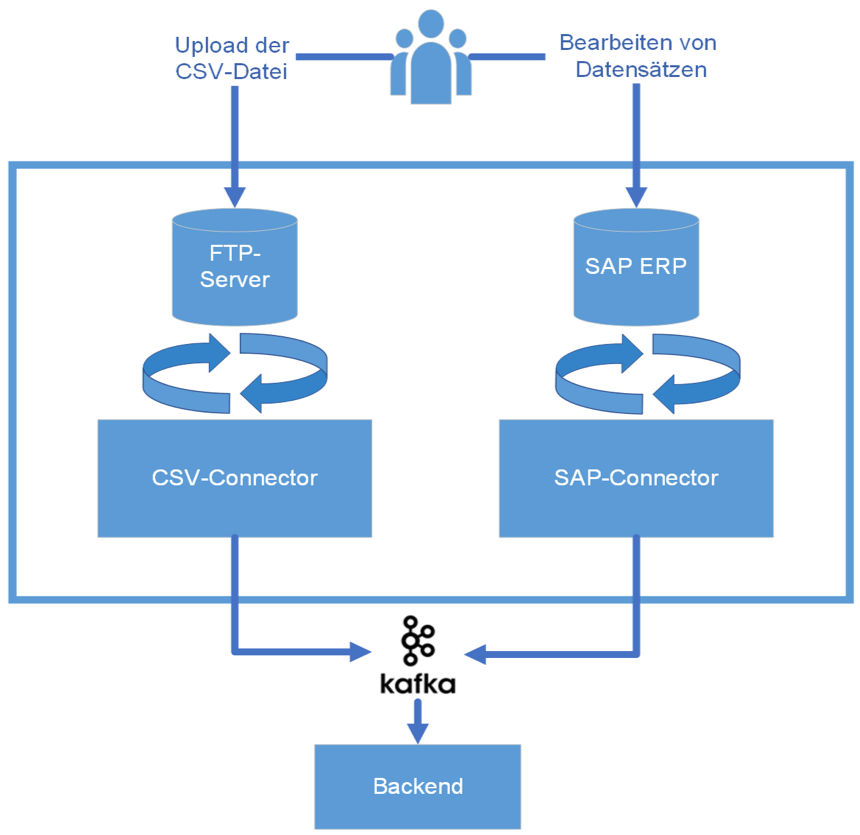
\includegraphics[width=\linewidth]{src/abbildungen/architektur_connector.png}
\newline
\captionof{figure}{Architektur der genutzten Konnektoren}
\newline

\subsection*{Funktionsweise der Konnektoren}
Nachdem die Anbindung über den JCo an den ABAP-Server hergestellt wurde, ist es möglich, Datenveränderungen auf dem ABAP-Server festzustellen. Wenn über die Oberfläche des ABAP-Servers direkt Daten verändert werden, kann die veränderte Tabelle mit Hilfe eines Outbound-Calls übermittelt werden.
\newline
Über Java werden für jede einzelne Zeile Datentransferobjekte erstellt, die dann an Kafka weitergeleitet werden.
\newline
\newline
Der SAP Java-Connector (JCo) ist eine Middleware-Komponente, die die Kommunikation zwischen Java-Komponenten und Java-Anwendungsservern mit dem SAP Server ABAP ermöglicht.
\newline
Durch einen Inbound-Call schickt der Java Client an den ABAP Server einen Request heraus. Die Antwort ist ein Outbound-Call des ABAP Servers an den Java Client.
\newline
So können Server und Client über Desktop- oder Serveranwendung miteinander kommunizieren.
\newline
\newline
Der CSV-Prozess erfolgt durch einen manuellen Import einer Datei auf den FTP-Server. Eine CSV-Datei wird auf den Server hochgeladen und im Hintergrund erfolgt eine regelmäßige Abfrage, ob Veränderungen zu der Altdatei festgestellt werden können. Sobald eine Veränderung erfolgt, werden auch hier mit Hilfe von Java Datentransferobjekte erstellt, die dann weiter an Kafka gesendet werden.
Die Datei wird dann dann automatisch aus dem Pfad des Ordners verschoben.

\section*{Was passiert im Hintergrund?}
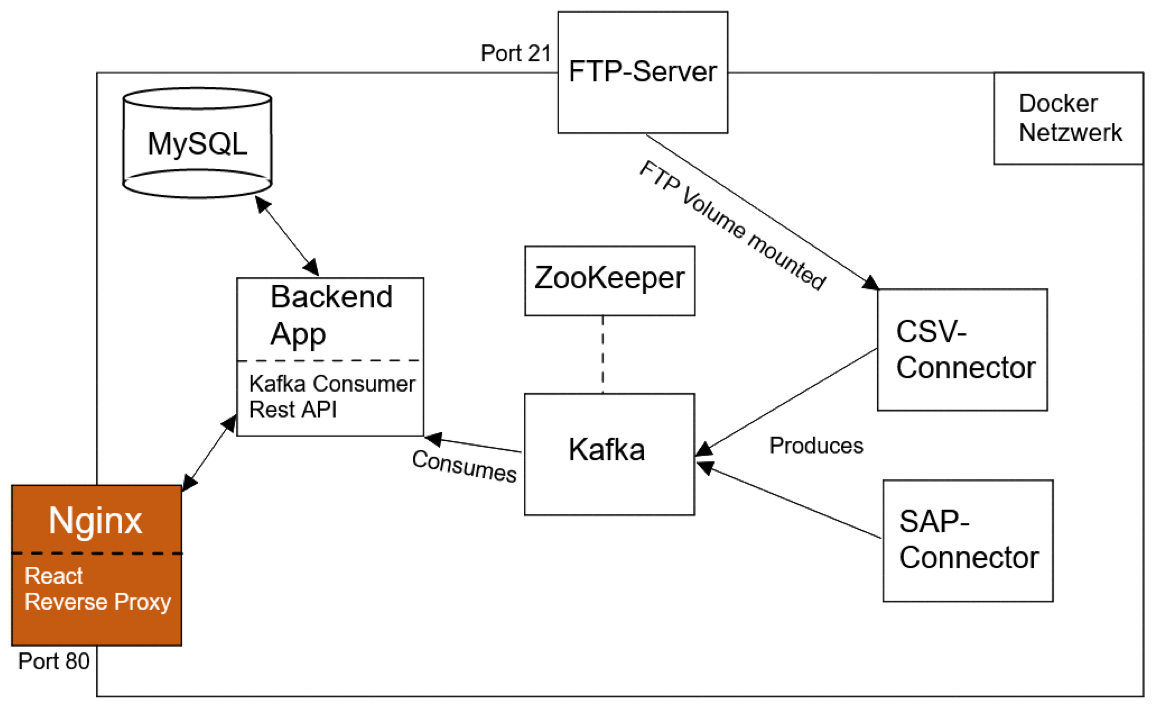
\includegraphics[width=\linewidth]{src/abbildungen/Architektur.png}
\captionof{figure}{Gesamtarchitektur zum Projektaufbau}
\newline
Um unser Ziel, Sales-Daten in Echtzeit zu visualisieren, müssen Frontend, Backend & das Live-Data-Monitoring bei Datenübertragungen etc. das gleiche Format nutzen.
\newline
\newline
Daher war es eine der Hauptaufgaben des Backends, zunächst einen ETL-Prozess aufzubauen, indem die Daten erfasst (Extraktion), im weiteren Verlauf transformiert und nach der Transformation also APIs bereitgestellt werden (Ladeprozess).
\newline


\section*{Angewendete Technologien}
Also Technologien kamen hauptsächlich ein gesammelter Java Stack bestehend aus dem Framework Spring Boot, Maven und Java selbst vor, um unter anderem die Anbindung der Konnektoren herzustellen.
\newline
Zudem nutzten wir neben Docker auch Kafka als Lösungstool, um uns vor den Problemen bei der langsamen Verarbeitung von großen Datensätzen zu schützen. Kafka ist ein sehr beliebtes Tool im Big-Data Umfeld und nutzt eigene Cluster. Kafka stellt Schnittstellen bereit, um große Datenströme in oder aus Drittsystemen zu importieren oder exportieren. (vgl. \cite{kafka2018})
\newline
\newline
Die Performance von Kafka ist ebenfalls gut. Bei unserem docker-basierten Setup wurden 130.000 Datentransferobjekte in knapp unter vier Sekunden an Kafka gesendet.
\newline
Für das Frontend nutzten wir die Technologien NginX, TypeScript, vite js und React.
\section*{Frontend}
\newline
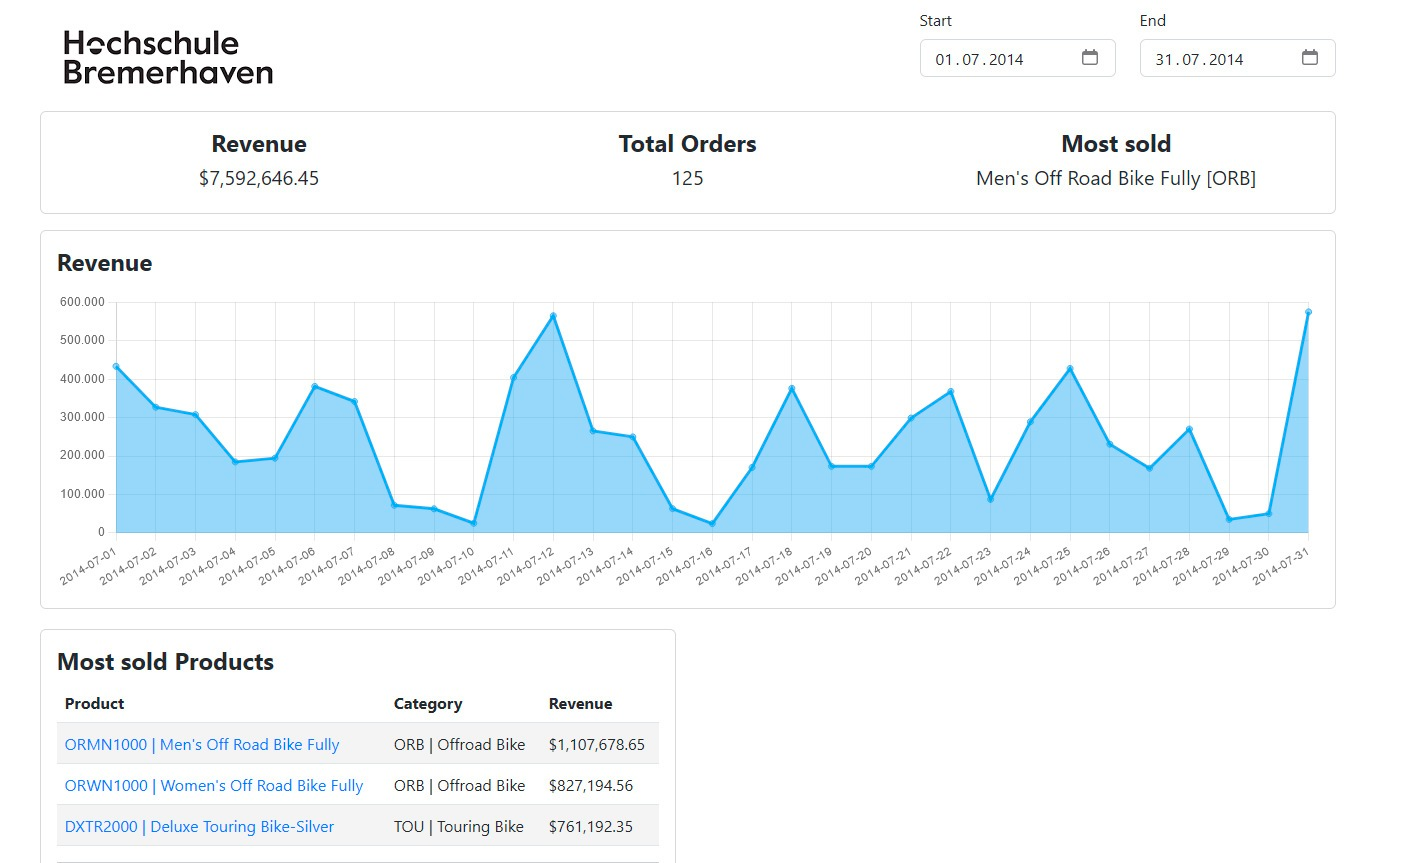
\includegraphics[width=\linewidth]{src/abbildungen/Frontend.png}
\captionof{figure}{Vorschaubild unserer Frontendanwendung}
\newline
\newline
\newline
Das Frontend stellt den visuellen Teil des Projektes dar. Der Nutzer kann die Daten, die vom Backend kommen, in Form von graphischer sowie tabellarischer Darstellung betrachten, diese individuell für seine persönlichen Zwecke auswerten und verwenden. Dabei besteht die Möglichkeit, verschiedene Abhängigkeiten und Zeiträume zu filtern.
\newline
\newline
Das Frontend wurde mittels folgender Technologien erstellt: React, ein entwicklerfreundliches und zukunftsorientiertes JavaScript Framework, TypeScript, eine Syntaxerweiterung für JavaScript und NginX, ein schneller Web-Server und Tool zur Einbindung eines ReverseProxys.
\newline
\newline
Ein Reverse Proxy ist ein Server, der für uns als Mittelsmann zwischen Client-Anfragen und dem eigentlichen Server agiert. Er empfängt Anfragen von Clients, leitet diese an den eigentlichen Server weiter und gibt die Antworten an den Client zurück. Dies kann verwendet werden, um die Sicherheit und Leistung der Anwendung zu erhöhen, indem es als Firewall dient, die Anfragen filtern kann, und indem es die Last auf mehrere Server verteilt.


\section*{Unser Projektfazit}
Das Projekt zur Entwicklung einer Live-Monitoring-Anwendung im SAP Bereich war für uns ein Erfolg. Wir haben uns in einem Zeitraum von zehn Monaten erfolgreich mit mehreren Technologien im SAP und Java Bereich auseinandersetzen können und viel Erkenntnisse gewinnen können.
\newline
\newline
Trotz einiger Herausforderungen konnten Komplikationen gemeisam bewältigt werden, indem sich in schwierigieren Situationen stets gegenseitig motiviert wurde. So war es für uns möglich, gemeinsam ein erfolgreiches Projekt abzuschließen.
\newline
\newline
Das Projektteam bestand aus 21 Personen, die alle ihre Stärken und Fähigkeiten eingebracht haben. Insgesamt war es eine großartige Erfahrung und ein sehr praxisnahes Projekt, das aus unserer Sicht ein wertvoller Beitrag zur Informatik an unserer Hochschule war.

  
    % Literaturverzeichnis anzeigen
    \phantomsection
    \renewcommand\refname{Literatur}
    \printbibliography

  \end{multicols*}
\end{document}

